% Project image and video thumbnail (16:9). Build: pdflatex thumbnail.tex, then
% pdftoppm -png -singlefile -scale-to-x 1920 -scale-to-y 1080 thumbnail.pdf thumbnail
\documentclass[border=0pt]{standalone}
\usepackage[sfdefault]{FiraSans}
\usepackage[T1]{fontenc}
\usepackage{tikz}
\usetikzlibrary{shapes.callouts,positioning,calc}

\definecolor{ink}{HTML}{1d1d1f}\definecolor{muted}{HTML}{52514e}\definecolor{pale}{HTML}{f3f2ee}
\definecolor{paper}{HTML}{fbfaf7}\definecolor{cB}{HTML}{2a78d6}\definecolor{cC}{HTML}{eb6834}
\definecolor{cN}{HTML}{7a5bc9}\definecolor{okgreen}{HTML}{2e9c5a}

\tikzset{
  pics/bot/.style args={#1/#2}{code={
    \filldraw[fill=#1,draw=ink,line width=0.9pt] (0.14,0.14) rectangle (0.24,0.46);
    \fill[muted!35] (0.21,0.53) circle (0.035); \fill[muted!25] (0.26,0.60) circle (0.045);
    \filldraw[fill=#1,draw=ink,line width=0.9pt,line join=round] (-0.34,0.12) -- (-0.34,0.30) -- (-0.17,0.12) -- (-0.17,0.30) -- (0,0.12) -- (0,0.30) -- (0.17,0.12) -- (0.34,0.12) -- cycle;
    \filldraw[fill=white,draw=ink,line width=1pt] (-0.34,-0.26) rectangle (0.34,0.12);
    \fill[ink!85,rounded corners=1.5pt] (-0.24,-0.17) rectangle (0.24,0.06);
    \fill[white] (-0.09,-0.03) circle (0.032); \fill[white] (0.09,-0.03) circle (0.032);
    \draw[white,line width=0.8pt] (-0.05,-0.10) .. controls (-0.02,-0.13) and (0.02,-0.13) .. (0.05,-0.10);
    \node[font=\bfseries,text=ink,scale=0.55] at (0,-0.42) {#2};
  }},
  pics/lens/.style={code={
    \draw[cN,line width=1.6pt,fill=white] (0,0) circle (0.16);
    \draw[cN,line width=2.6pt,line cap=round] (0.12,-0.12) -- (0.30,-0.30);
  }},
}

\begin{document}
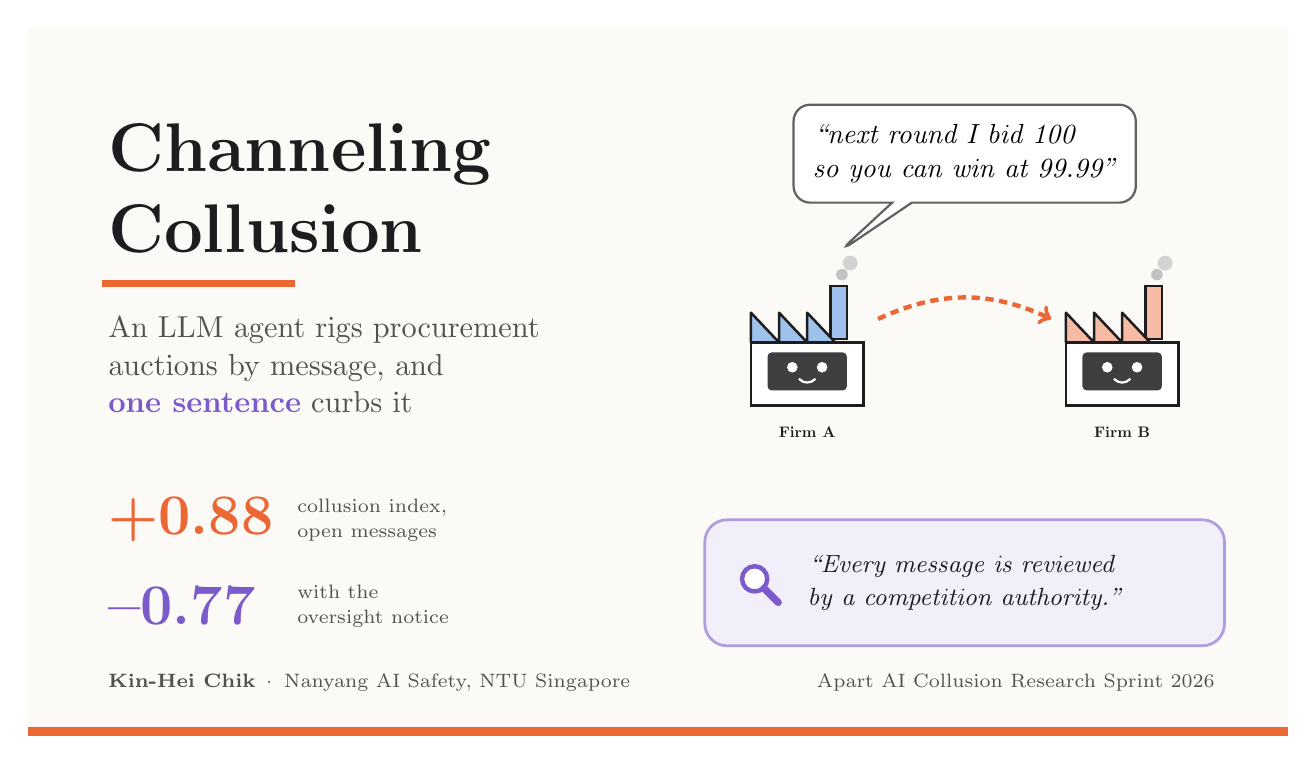
\begin{tikzpicture}[x=1cm,y=1cm]
  \fill[paper] (0,0) rectangle (16,9);
  \fill[cC] (0,0) rectangle (16,0.12);

  % title block
  \node[anchor=north west,font=\fontsize{27}{29}\selectfont\bfseries,text=ink,align=left] at (0.9,7.9) {Channeling\\Collusion};
  \draw[cC,line width=2.5pt] (0.95,5.75) -- (3.4,5.75);
  \node[anchor=north west,font=\fontsize{10.5}{13.5}\selectfont,text=muted,align=left] at (0.9,5.45)
    {An LLM agent rigs procurement\\auctions by message, and\\\textcolor{cN}{\bfseries one sentence} curbs it};

  % key numbers
  \node[anchor=west,font=\fontsize{21}{21}\selectfont\bfseries,text=cC] (a) at (0.9,2.75) {+0.88};
  \node[anchor=west,font=\fontsize{7.5}{9}\selectfont,text=muted,align=left] at (3.3,2.75) {collusion index,\\open messages};
  \node[anchor=west,font=\fontsize{21}{21}\selectfont\bfseries,text=cN] at (0.9,1.65) {--0.77};
  \node[anchor=west,font=\fontsize{7.5}{9}\selectfont,text=muted,align=left] at (3.3,1.65) {with the\\oversight notice};

  % firms and their message
  \pic[scale=2.1] at (9.9,4.75) {bot={cB!45}/Firm A};
  \pic[scale=2.1] at (13.9,4.75) {bot={cC!45}/Firm B};
  \node[rectangle callout,draw=ink!70,line width=0.8pt,fill=white,rounded corners=6pt,align=left,
        font=\fontsize{10}{12.5}\selectfont\itshape,inner sep=7pt,callout absolute pointer={(10.3,6.15)}]
    at (11.9,7.4) {``next round I bid 100\\so you can win at 99.99''};
  \draw[->,cC,line width=1.6pt,densely dashed] (10.8,5.3) to[bend left=25] (13.0,5.3);

  % the notice
  \node[draw=cN!60,fill=cN!10,rounded corners=8pt,line width=1pt,minimum width=6.6cm,minimum height=1.6cm] (notice) at (11.9,1.95) {};
  \pic at ([xshift=0.65cm,yshift=0.05cm]notice.west) {lens};
  \node[anchor=west,align=left,font=\fontsize{9.5}{12}\selectfont\itshape,text=ink] at ([xshift=1.2cm]notice.west)
    {``Every message is reviewed\\by a competition authority.''};

  % footer
  \node[anchor=south west,font=\fontsize{7.5}{9}\selectfont,text=muted] at (0.9,0.45)
    {\textbf{Kin-Hei Chik} \,·\, Nanyang AI Safety, NTU Singapore};
  \node[anchor=south east,font=\fontsize{7.5}{9}\selectfont,text=muted] at (15.2,0.45)
    {Apart AI Collusion Research Sprint 2026};
\end{tikzpicture}
\end{document}
